\batchmode
\documentclass[a4paper,10pt]{article}
\usepackage{graphicx}
\usepackage{fancyvrb}
\usepackage{color}
\usepackage{xcolor}
\usepackage{verbatim}
\usepackage{amssymb}
\usepackage{amsmath}
\usepackage{hyperref}
\usepackage{natbib}
\usepackage{caption}
\usepackage{subcaption}

\hypersetup{urlcolor=blue, colorlinks=true}
\usepackage{float}

%used in SL section
\usepackage{mathptmx}
\usepackage{siunitx} %SI-einheiten
\usepackage{lmodern} %weitere mathematischen Symbole
\usepackage{placeins} %floatbarrier

\DeclareSIUnit\parsec{pc}
\DeclareSIUnit\lightyear{ly}
\DeclareSIUnit\year{yr}
\DeclareSIUnit\erg{erg}
\DeclareSIUnit\ster{ster}
\DeclareSIUnit\arcsec{arcsec}
\DeclareSIUnit\deg{deg}


\definecolor{gruen}{cmyk}{0.35,0.01,0.80,0.1}

\textheight=25.5cm
\textwidth=17.5cm
\voffset=0.cm
\hoffset=-0.0cm
\oddsidemargin -1cm
\evensidemargin -1cm
\topmargin -2cm
\baselineskip=0.900cm
\setlength{\parindent}{0in}

\graphicspath{{../figures/}}

\providecommand{\e}[1]{\ensuremath{\times 10^{#1}}}
\newcommand{\given}[2]{\ensuremath{P(#1|#2)}}
\newcommand{\x}[0]{\ensuremath{\vec{x}}}
\newcommand{\gauss}[3]{\ensuremath{\frac{1}{\sqrt{2\pi#2^2}}\text{exp}\left(- \frac{(#1-#3)^2}{2#2^2}\right)}}

% used in SL section
\newcommand{\todo}[2]{\textcolor{red}{\textbf{TODO (#1): #2}}}

\title{Serendipitous Detections of Kilonovae}
\author{Authors: Christian N. Setzer\footnote{christian.setzer@fysik.su.se} , Rahul Biswas, Hiranya V. Peiris}
\date{}


\begin{document}
\maketitle

The metric we have chosen for evaluation of a cadence is the number of KNe that are detected given the simulations of observations we have conducted. The criteria that we use to determine detections is that of \citet{Scolnic2017a}. These criteria are the following:
\begin{itemize}
  \item Two alerts separated by $\geq 30$ minutes.
  \item Observations in at least two filters with $\mathrm{SNR} \geq 5$.
  \item Observations with $\mathrm{SNR} \geq 5$ separated by maximum 25 days.
  \item A minimum of one observation of the same location within 20 days before the first $\mathrm{SNR} \geq 5$ observation.
  \item A minimum of one observation of the same location within 20 days after the last $\mathrm{SNR} \geq 5$ observation.
\end{itemize}

In this context an alert is an observation that has a measured signal-to-noise ratio greater than five after template subtraction. This is simulated using the per-filter efficiency vs. true signal-to-noise ratio response function. As this function is unknown for LSST prior to operation, we have used the set of functions that were adopted for the DES Y1 analysis, given their filter-set is similar to LSST [R. Kessler, private communication]. The observations are filtered according to these criteria and the subset of transients which pass all conditions are labeled as detections.

These are the detection results for kilonovae using a single realization of the redshift distribution for each cadence. Each of these is itself a draw from a Poisson distribution as explained above. The uncertainty on these values is then the square root of the sample mean. For the case of one sample, this mean is the number of detections that are found per cadence, and the uncertainty on the number of detections is the square root of the numbers of detections.
\begin{figure}[h!]
  \centering
  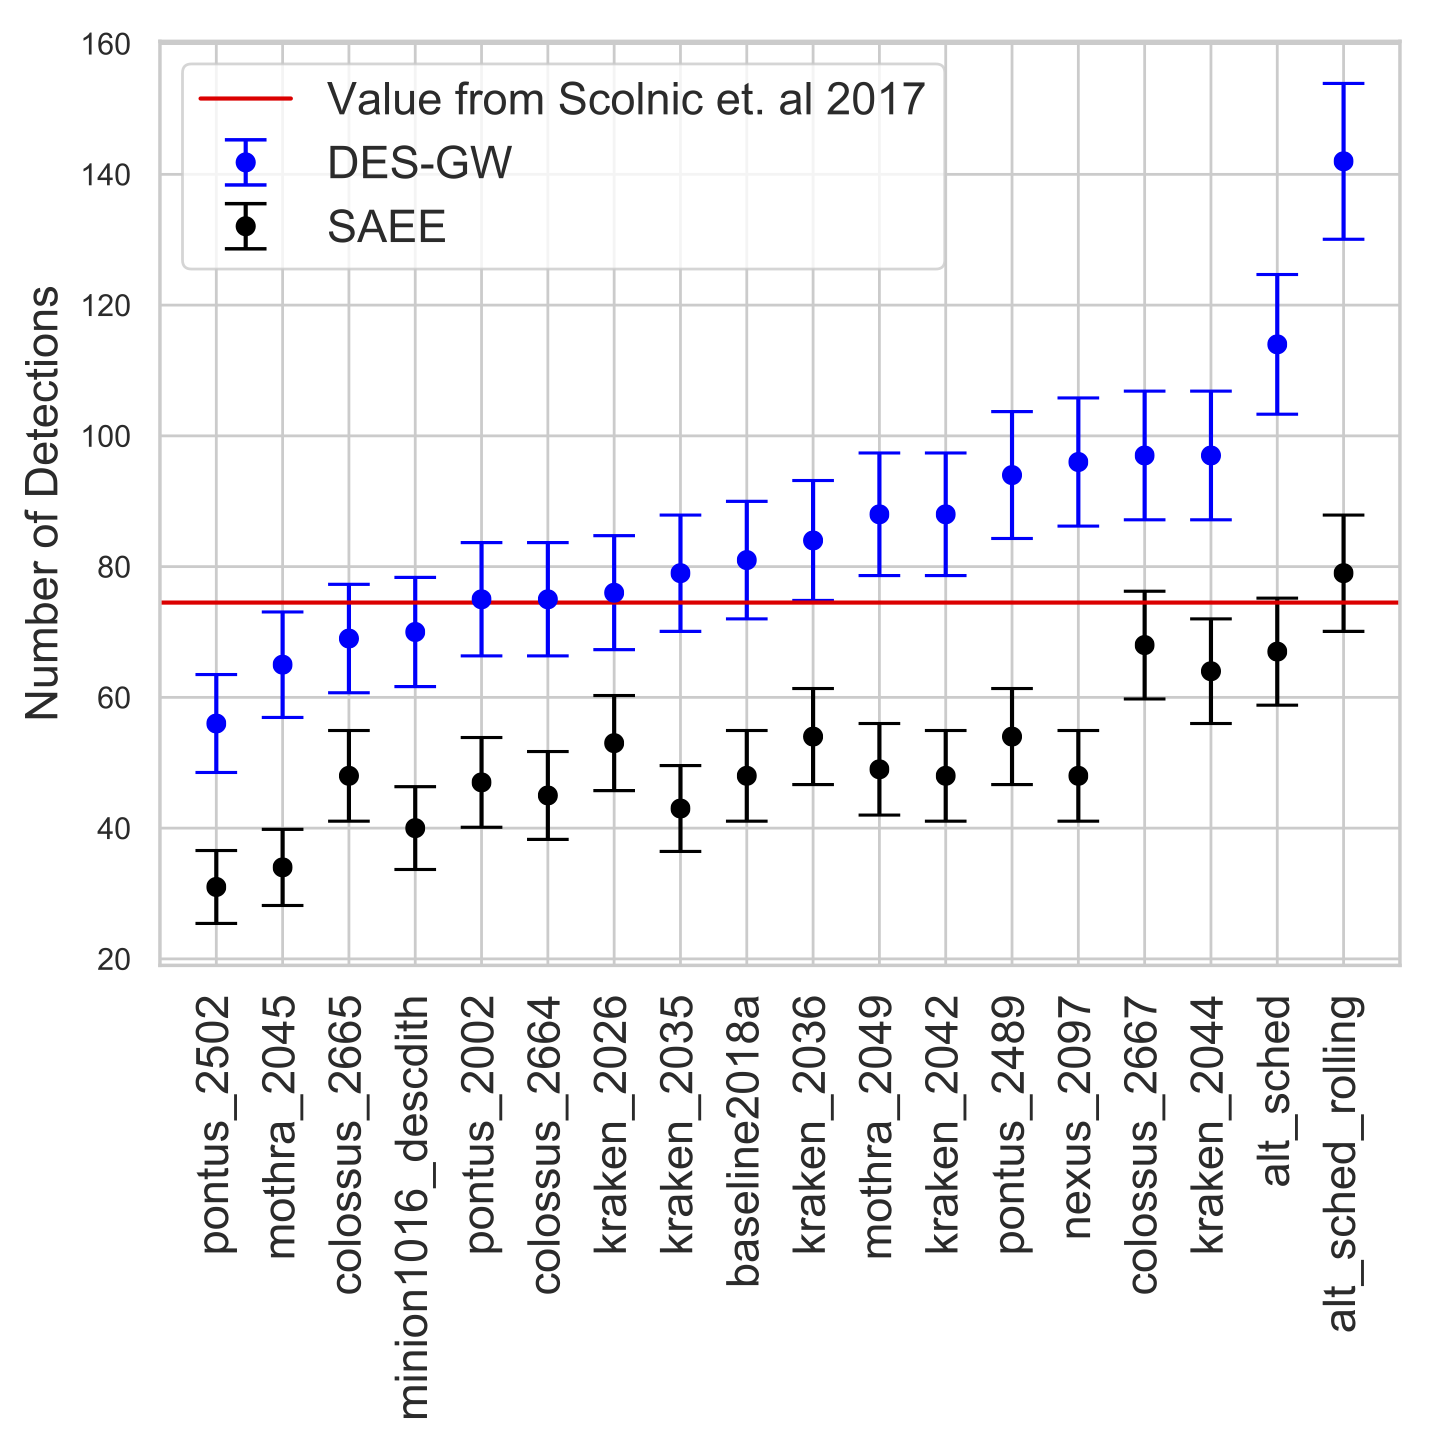
\includegraphics[scale=0.69]{../figures/total_detection_counts_by_cadence}
  \caption{Ranking of cadence strategies for both KNe models, based on the total number of detections found in both the WFD and DDF parts of each cadence.}
  \label{fig:cadence_ranking}
\end{figure}

%Most summaries shouldn't need references as it's just a description of the metric. Refs should be in the main DESC note
\bibliographystyle{unsrt}
\bibliography{../refs}


\end{document}
